\chapter{Current methods of comparing rasters}

When trying to solve an issue it is important to understand what the current methods for achieving the same is. This chapter will present three current methods for comparing rasters.

\section{Desktop Gis program}

One way of visualising the population data would be to load the data into a desktop GIS programs like QGIS or ArcGIS. Both of these can visualise TIFF files and it is possible to visually compare different raster layers by changing back and fourth between the different layers. However one would have to manually style the layer to make spatial patterns become visible. Without styling the layer the tiff file will be colorized based on the most and least populated areas in the world. When coloring based on these extremes most of the world will appear in the same color as illustrated in figure \ref{QGIS}. Only the most populated areas in India and china will appear in a different color. This is further expanded upon in section \fxnote{Ref to core concepts}

\fxnote{Remember Carsten mail about locally, on-the-fly and subdomains}
\begin{figure} [H]
	\centering
	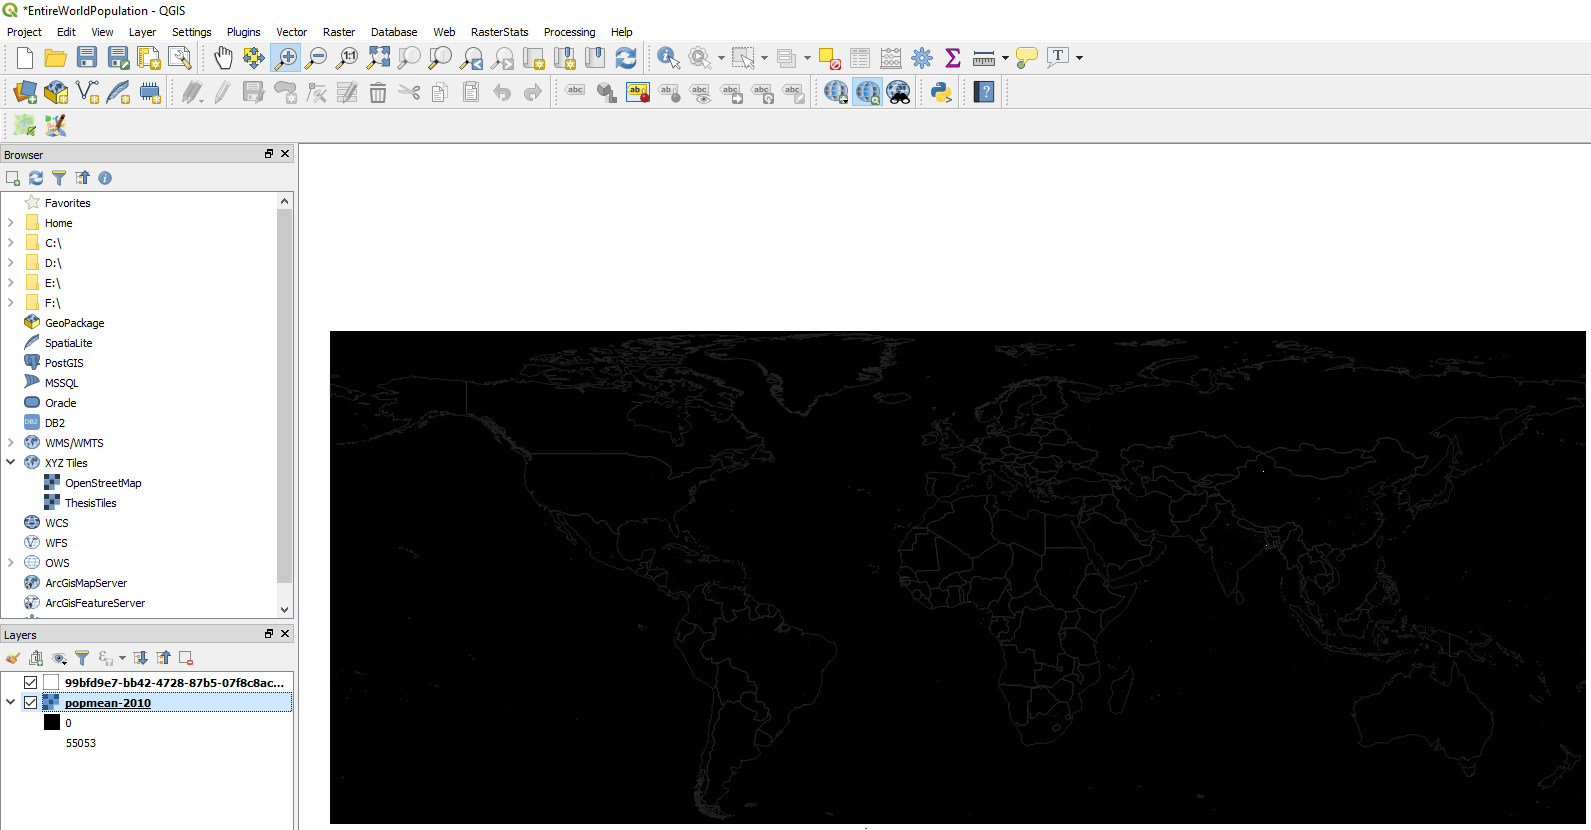
\includegraphics[width=.8\textwidth]{Pictures/QGIS}
	\caption{The population distribution visualised in QGIS and colored based on data from the entire world}
	\label{QGIS}
\end{figure}

\section{Interactive visualization tool for population simulations}

\begin{figure} [H]
	\centering
	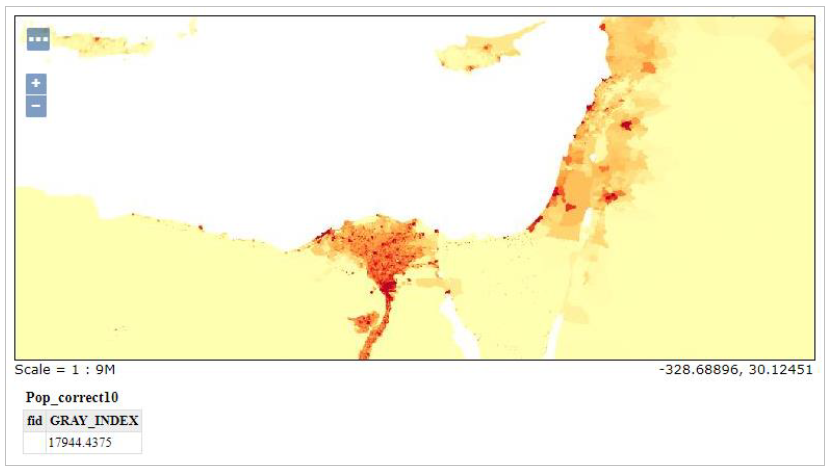
\includegraphics[width=.8\textwidth]{Pictures/Geoserver}
	\caption{An interactive visualization tool made in GeoServer showing the population near Cairo. Source: \citet{Sarah}}
	\label{Geoserver}
\end{figure}

\citet{Sarah} wrote a her master thesis about interactive visualisation of the same population projections, which is the case data for this project. In the thesis she tests different methods for interactive visualisation. The first tests are the python libraries Bokeh and Folium. Both of these are creating interactive webbased maps, but were unable to visualize the population projects due to the file size of the rasters. Therefore other solutions were created using servers for geographic imagery. The servers GeoServer and MapServer were used in the thesis, which both uses Openlayers for their interactive interface. Figure \ref{Geoserver} shows the Geoserver visualisation of the raster data. Figure \ref{Mapserver} shows the Mapserver solution. Both tools required a manual styling.

\begin{figure} [H]
	\centering
	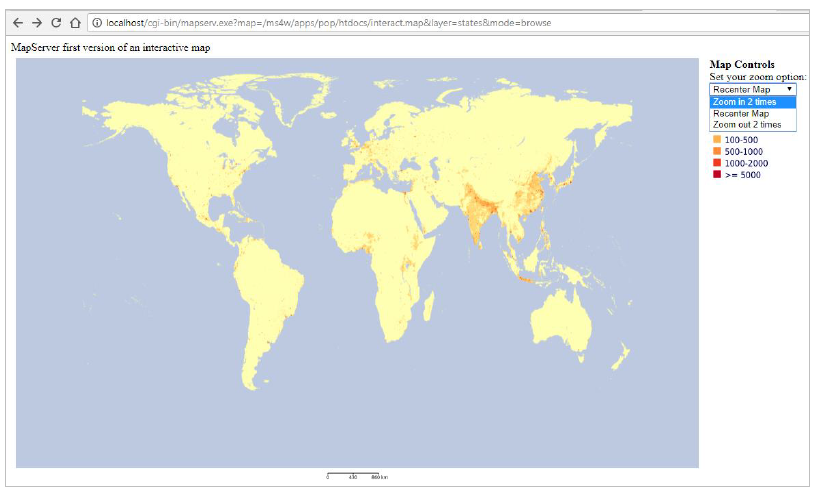
\includegraphics[width=.8\textwidth]{Pictures/Mapserver}
	\caption{An interactive visualization tool made in MapServer. Source: \citet{Sarah}}
	\label{Mapserver}
\end{figure}

The conclusion in the thesis was that MapServer was the faster option, whereas GeoServer was easier to learn. Using either server were slower than viewing in QGIS. Both had limited customizability. As shown in the two figures the tool were only showing a single map and not having and interface for changing the raster layers. The tools were therefore more of a visualization tool, than a comparison tool.


%Sarah 19

\section{MakeCityWebsite}
One of the creators of the case data created a python script, called MakeCityWebsite, for comparing the different population projections for a chosen city.  The final product of the tool can be seen in figure x and x. 

\begin{figure} [H]
	\centering
	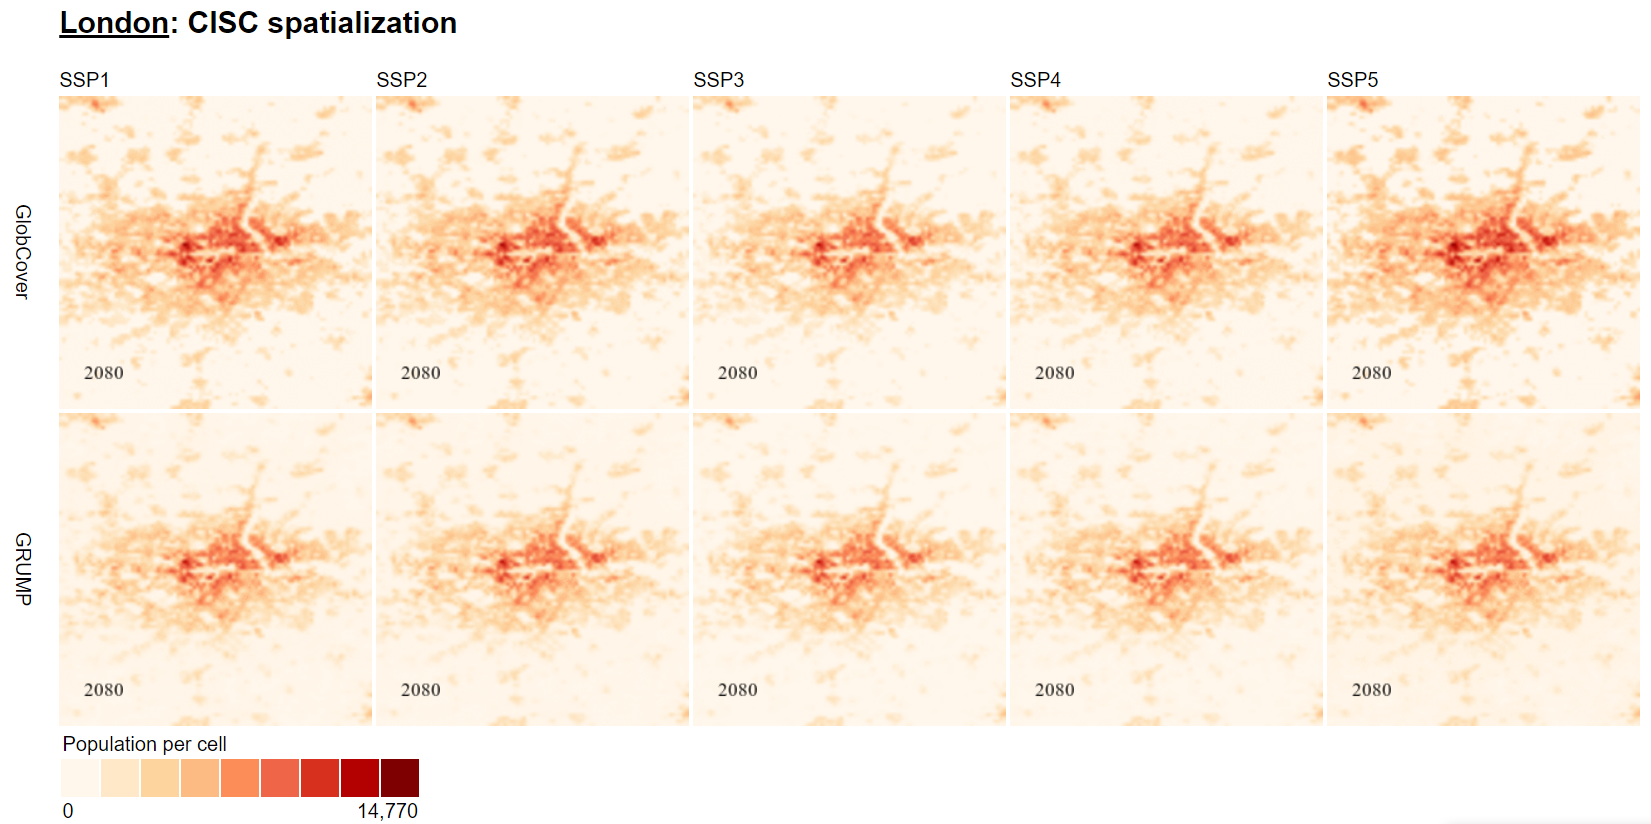
\includegraphics[width=.8\textwidth]{Pictures/MakeCityWebsite1}
	\caption{The output of running the MakeCityWebsite script for London. Each population density map is a gif based on different combinations of urbanization model and scenario. The other pictures in the gif are other years}
	\label{MakeCityWebsite1}
\end{figure}
\fxnote{Update fig text to be independed}

\fxnote{Top part of figure looks more populated. Should be opposite? Maybe a lot of infrastructure}
The input for the tool is the rasters from each of the two urbanization models, the five SSPs and every tenth year from 2010-2100, so a total of hundred different rasters.
The tool first create new raster files, which have been cut to the extent of the chosen city. Then the minimum and maximum value in those file are calculated. The maximum and minimum values among all the rasters are then used to determine a color scale. This color scale is then used to create a new set of colored rasters.

So at this point the tool have generated one hundred rasters, which all have been colored using the same color scale. For the user to be able to comprehend this amount of data two additional steps are taken. First the individual combinations of urbanization models and SSPs are collected in gifs. These gifs are displayed how the population evolve in their scenario by chronology changing between different years. These different gifs are then placed next to each other in a website as illustrated in figure x. 

\begin{figure} [H]
	\centering
	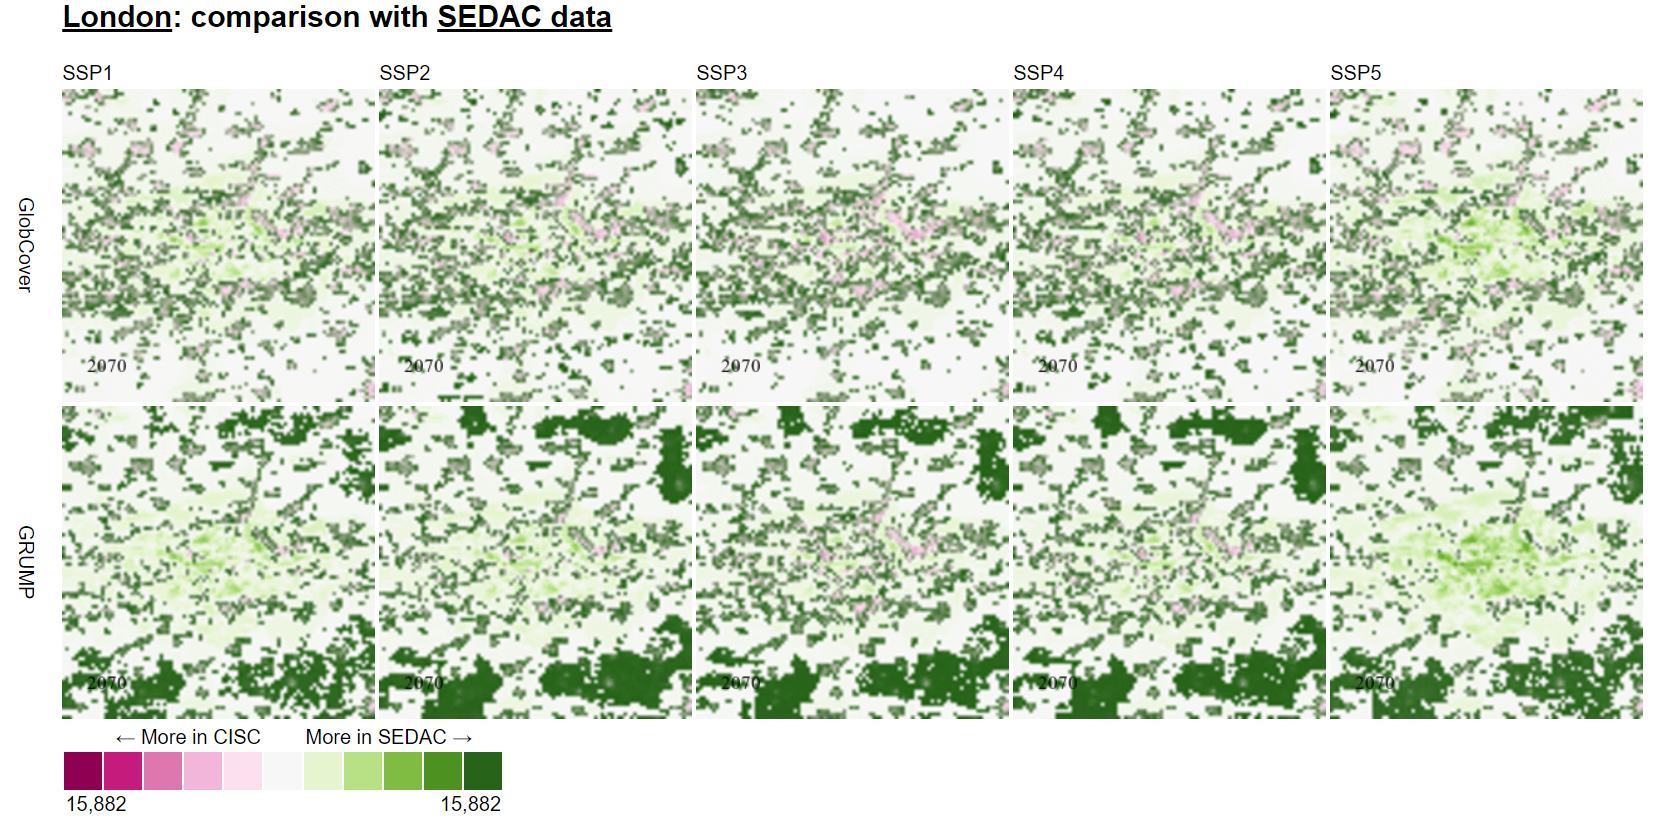
\includegraphics[width=.8\textwidth]{Pictures/MakeCityWebsite2}
	\caption{MakeCityWebsite also creates a comparison with another population projection called SEDAC. Each map shows the difference in values between the two population projection for each combination of urbanization model and scenario.}
	\label{MakeCityWebsite1}
\end{figure}
\fxnote{Is Sedac based on the same data as carstens?? - is sedac a pop projection or do I need another term}
The tool also creates a comparison with other another population projection called SEDAC. This is done by going though the same steps above, but with a custom raster. This raster visualise the difference between the two projection. This comparison part of the website can be seen in figure z
https://github.com/crstn/CISC/blob/master/MakeCityWebsite.py

The creation of these comparison rasters take 20 minutes for a single SSP
https://github.com/crstn/CISC/blob/master/CompareWithSEDAC.py

\fxnote{How long time does it take to run MakeCityWebsite}



